\section{Art Style}
The art style of \ourgame{} is largely influenced by the individual styles and previous works of \ourteam{}'s art department.

\begin{figure}[H]
\centering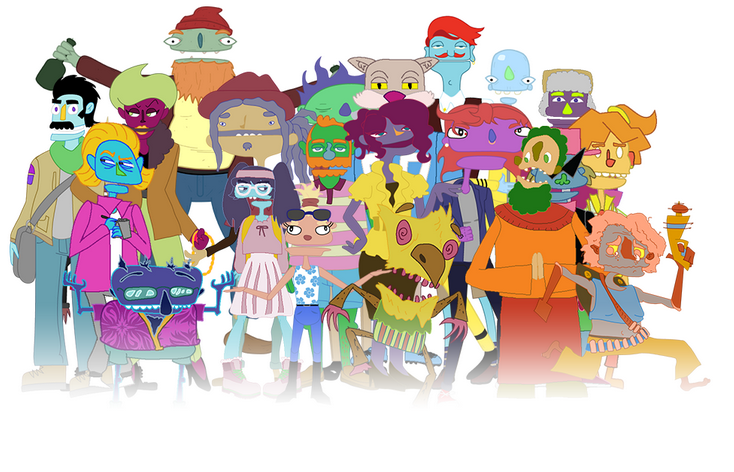
\includegraphics[width=0.7\linewidth]{images/art_style}
\end{figure}

\clearpage
\subsection{Michael}
Michael's artistic tendencies lean toward sharp and angular shapes. His characters tend to be more lanky and creepy. Limbs were generally long and thin. uniform in thickness. The colours usually used are dark earthy tones. \ourgame{}'s character's art style and concepts were mainly inspired by Michael's art for a previous game, \textit{"This Is Our Game And I'm Out Of Ideas"}, seen in Figure~\ref{fig:m3}, where characters were broken into components and moved strangely, possessing inhuman freedom in joint movement. 

\begin{figure}[H]
  \centering\begin{subfigure}{.5\textwidth}
    \centering
    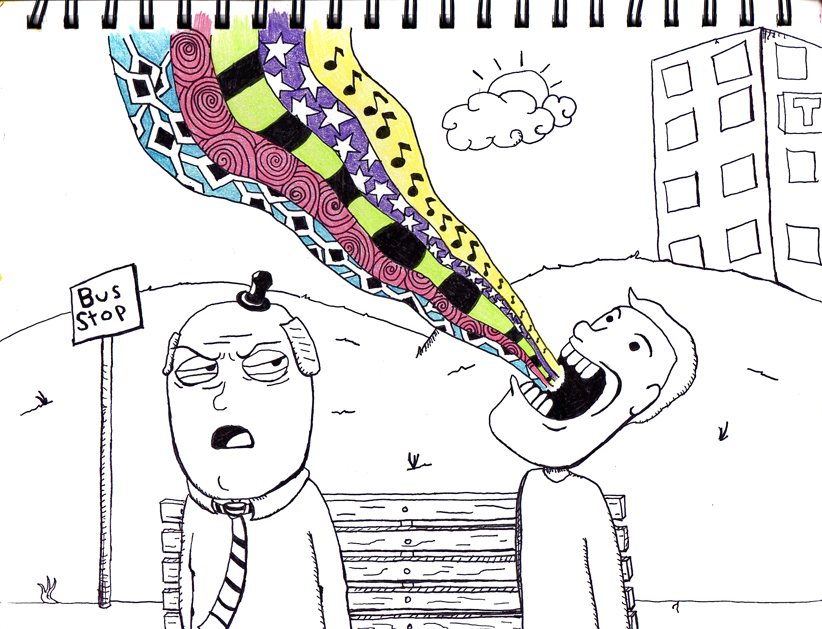
\includegraphics[width=.9\linewidth]{images/ref_MICHAEL02}
  \end{subfigure}
  \begin{subfigure}{.45\textwidth}
    \centering
    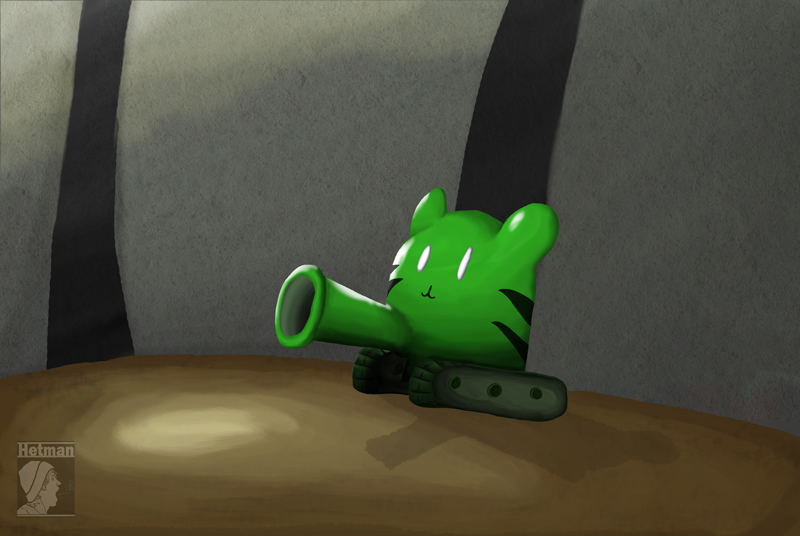
\includegraphics[width=.9\linewidth]{images/ref_MICHAEL01}
  \end{subfigure}
  \begin{subfigure}{.5\textwidth}
    \centering
    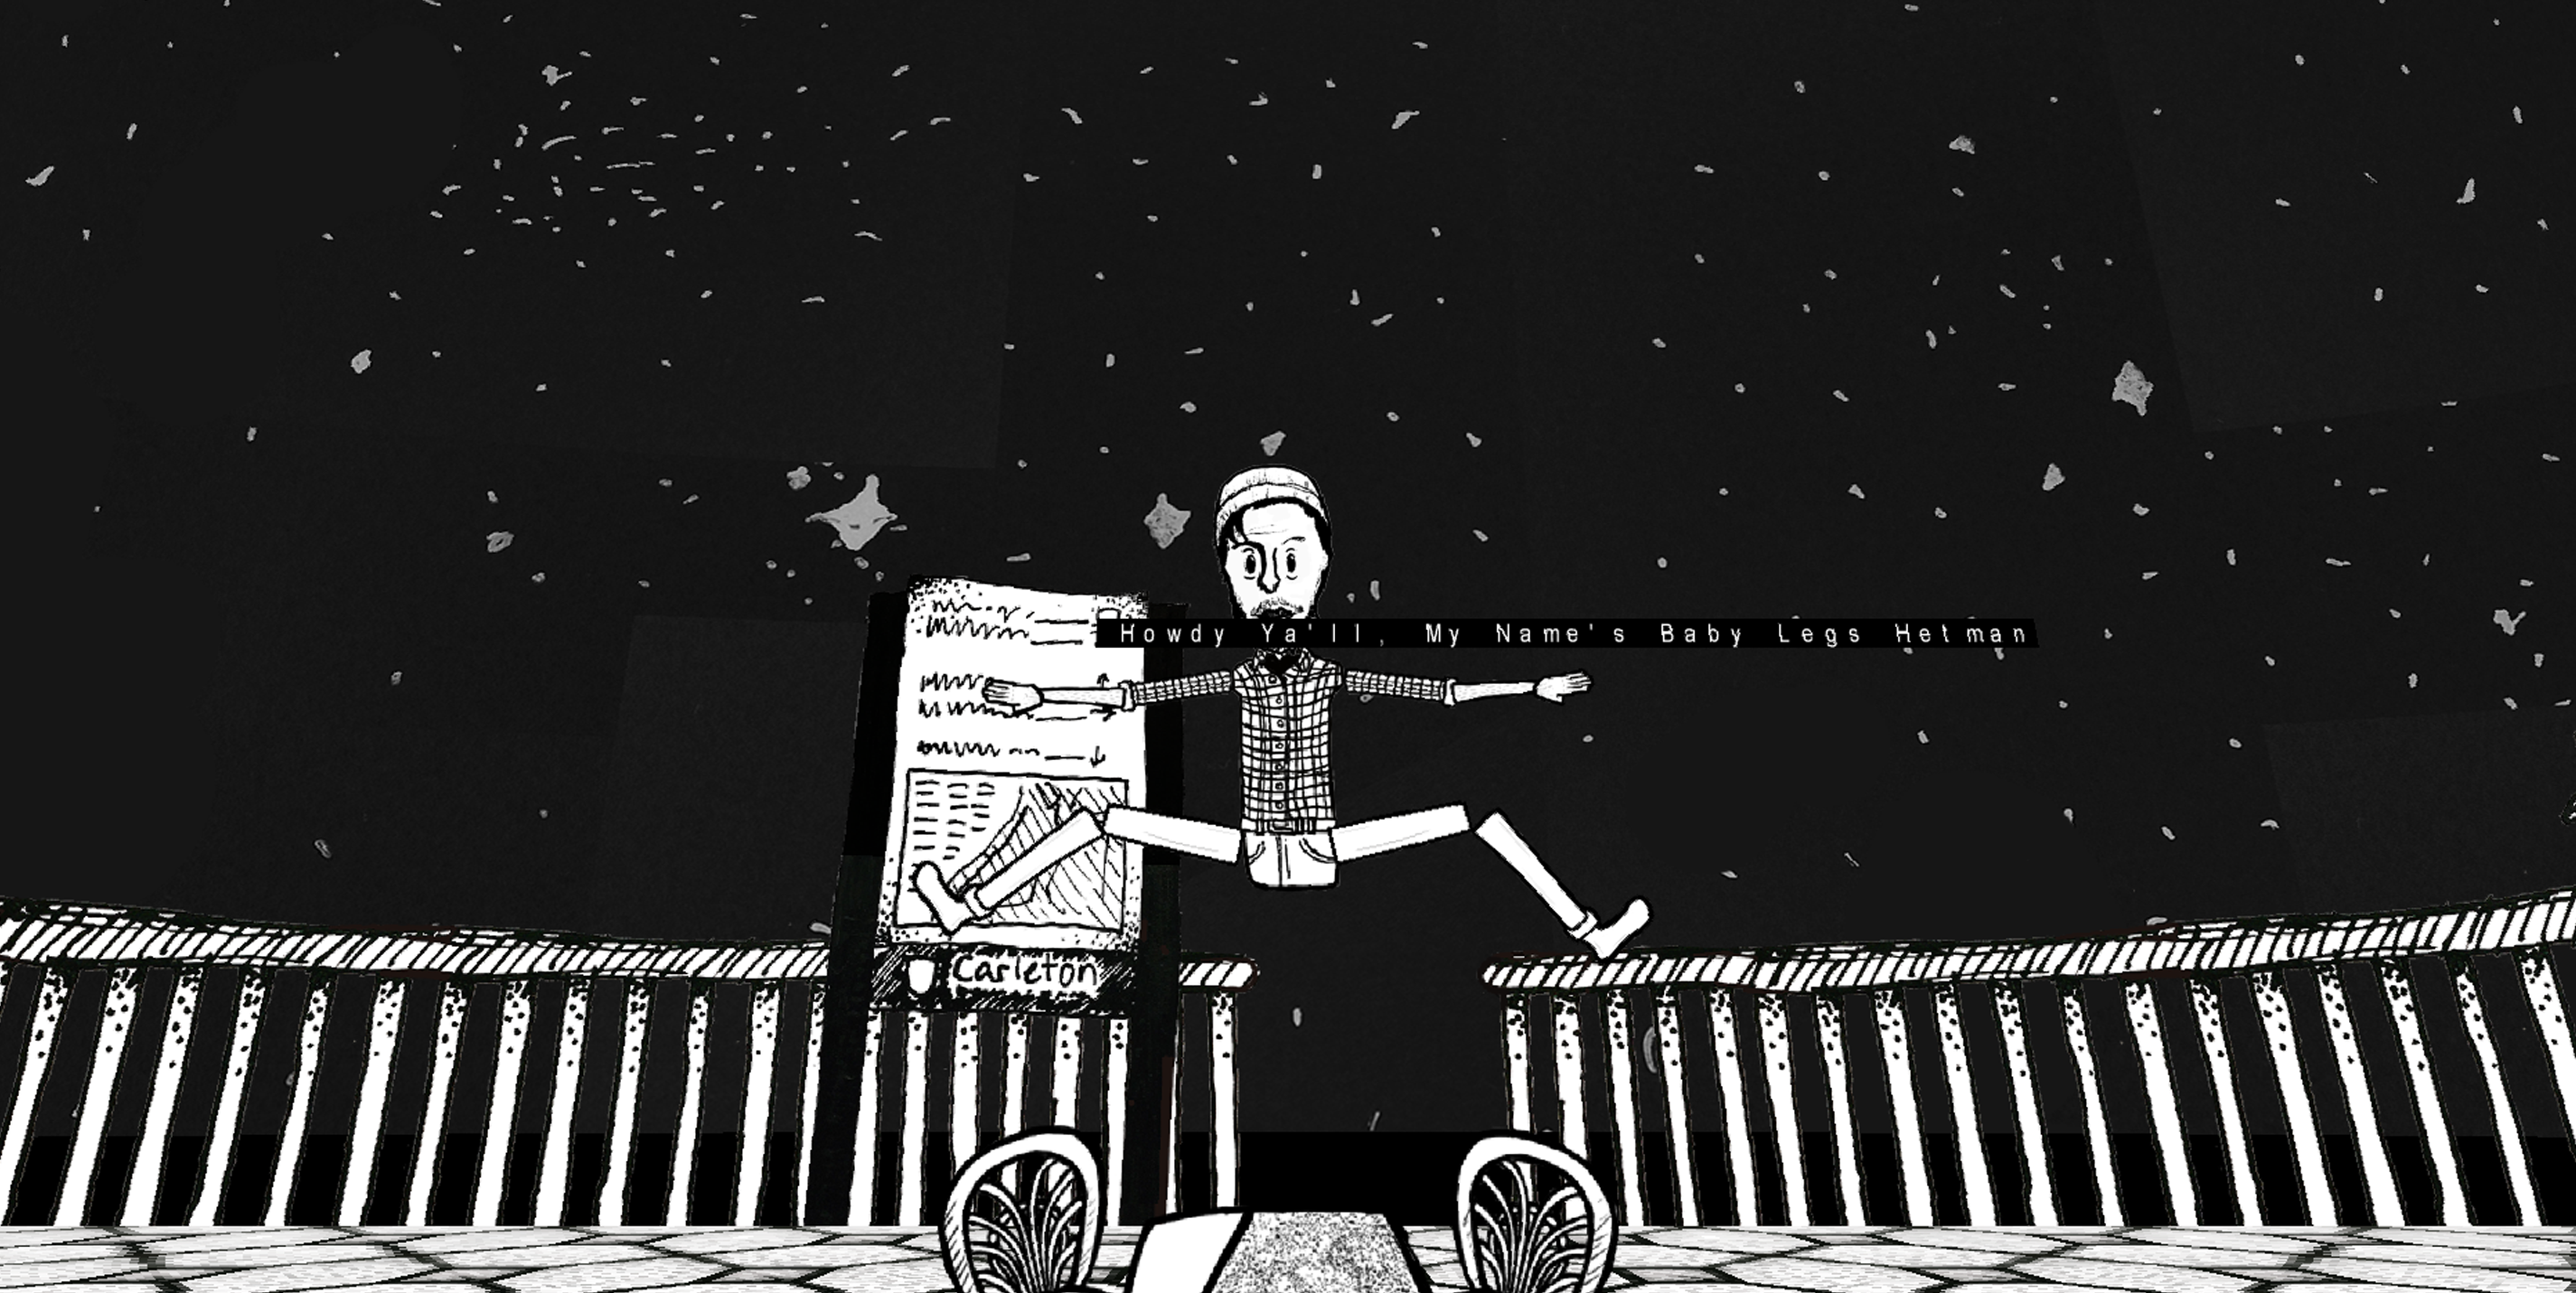
\includegraphics[width=.9\linewidth]{images/ref_MICHAEL03}
    \caption{Character in TIOGAIOOI}
    \label{fig:m3}
  \end{subfigure}
  \begin{subfigure}{.45\textwidth}
    \centering
    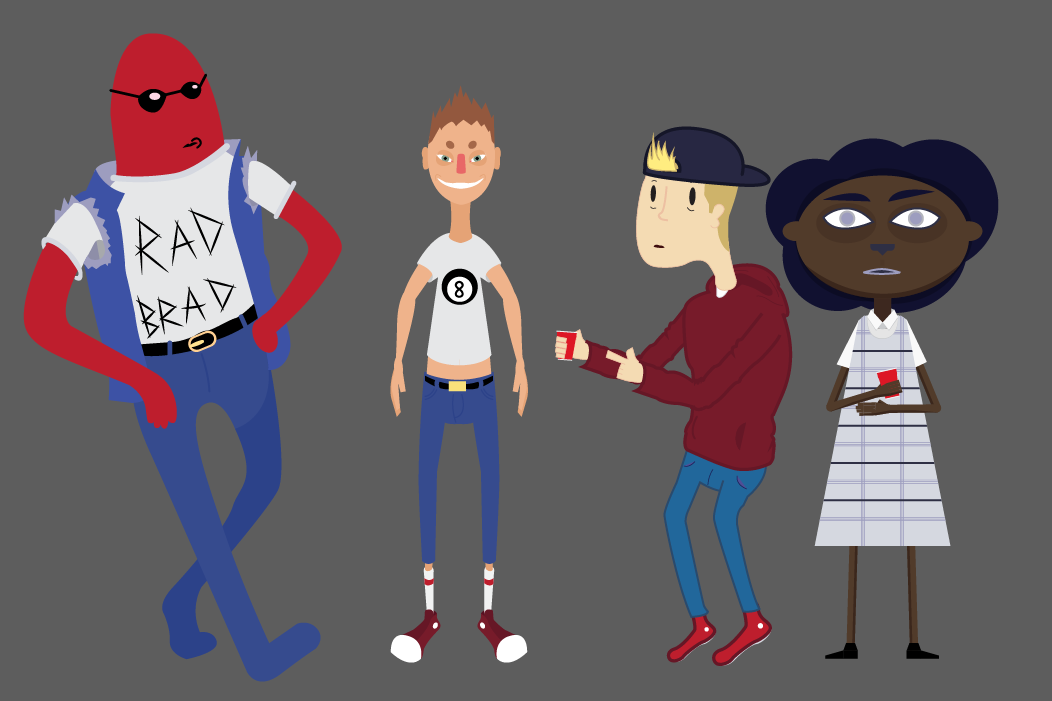
\includegraphics[width=.9\linewidth]{images/ref_MICHAEL04}
    \caption{Initial Character Ideas}
    \label{fig:m4}
  \end{subfigure}
  \caption{Michael's Art Style}
  \label{fig:mstyle}
\end{figure}

\clearpage
\subsection{Sean}
Sean's art style is fluid, whimsical and creative. His characters cover a wide range of monster and creature based designs, some of which are non-humanoid and non-bipedal. There is a certain appeal to the beings he creates, as their expressions are evident and viewer can relate. The same can be said for his human characters. He prefers to doodle ideas and illustrate creations of his imagination which are stylized with a nostalgic storybook illustration style.

\begin{figure}[H]
  \centering\begin{subfigure}{.5\textwidth}
    \centering
    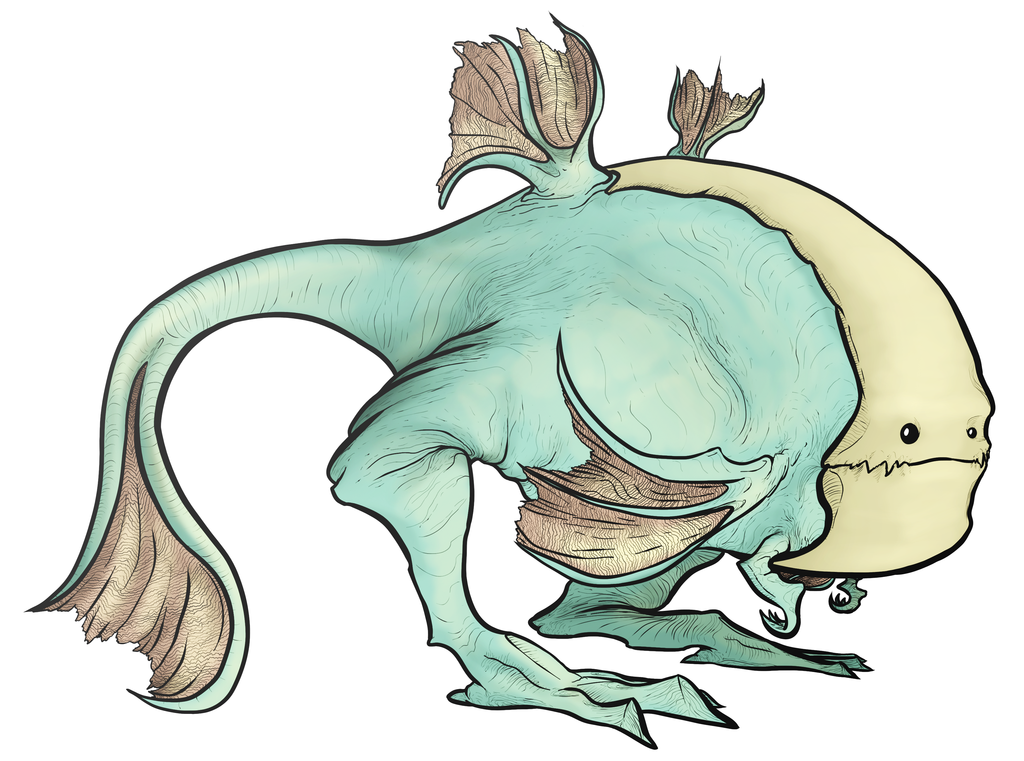
\includegraphics[width=.9\linewidth]{images/ref_SEAN01}
  \end{subfigure}
  \begin{subfigure}{.11\textwidth}
    \centering
    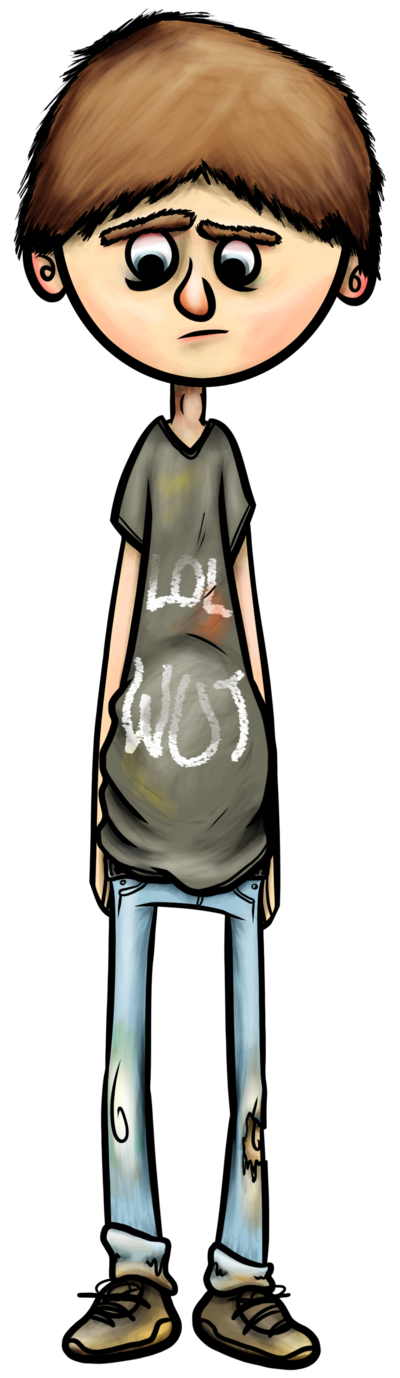
\includegraphics[width=.9\linewidth]{images/ref_SEAN02}
  \end{subfigure}
  \\
  \begin{subfigure}{.3\textwidth}
    \centering
    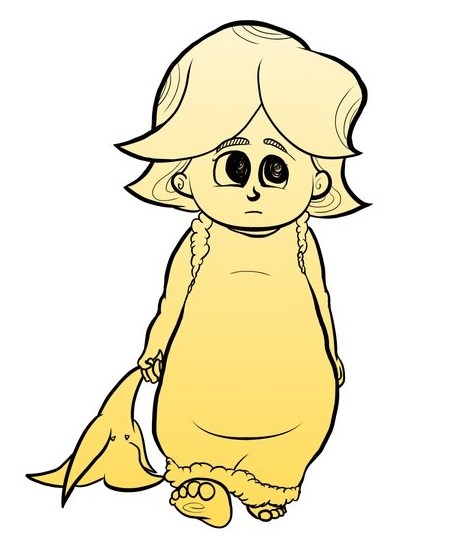
\includegraphics[width=.9\linewidth]{images/ref_SEAN03}
  \end{subfigure}
  \begin{subfigure}{.3\textwidth}
    \centering
    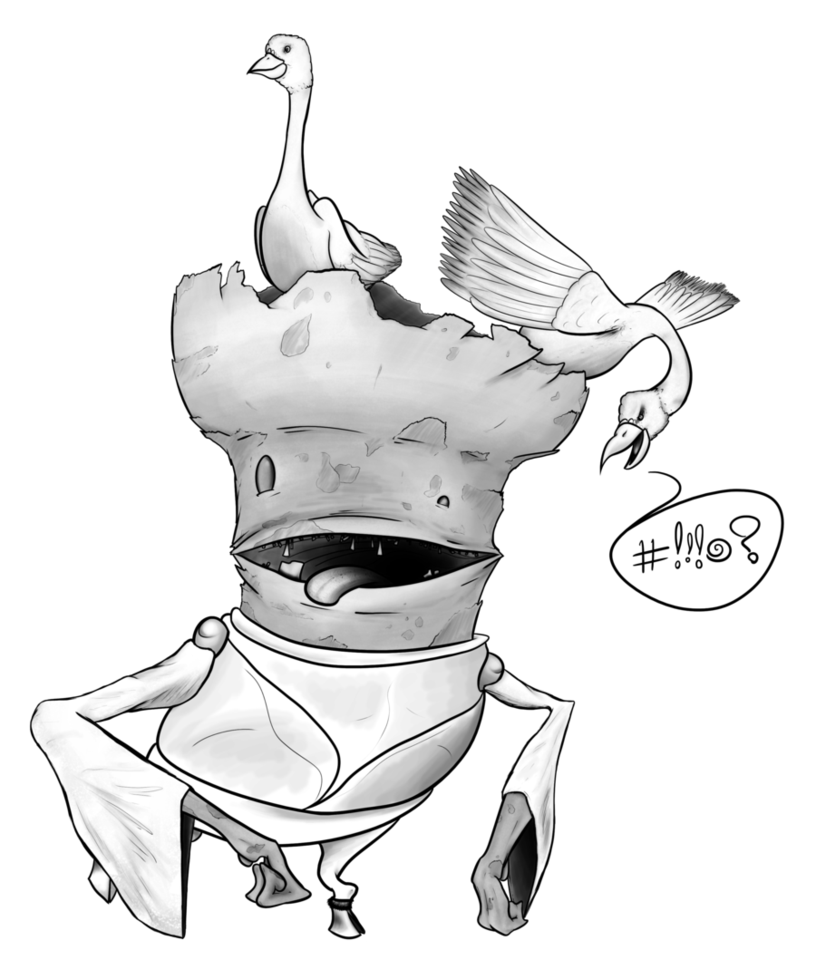
\includegraphics[width=.9\linewidth]{images/ref_SEAN04}
  \end{subfigure}
  \caption{Sean's Art Style}
  \label{fig:sstyle}
\end{figure}

\clearpage
\subsection{Ian}
Ian's approach to art is more curvaceous, smooth and delightful. His characters, while incorporating otherworldly features, are designed in a certain way that is grounded in the real world. He enjoys designing characters that would fit in perfectly in an alternate universe. Anthropomorphic and folklore themes are prevalent his cartoon-like characters, presented as mundane beings sporting modern clothing. The character styles from one of his comics, shown in Figure~\ref{fig:i1}, were a starting point from which \ourgame{}'s character designs stemmed from.

\begin{figure}[H]
  \centering\begin{subfigure}{.4\textwidth}
    \centering
    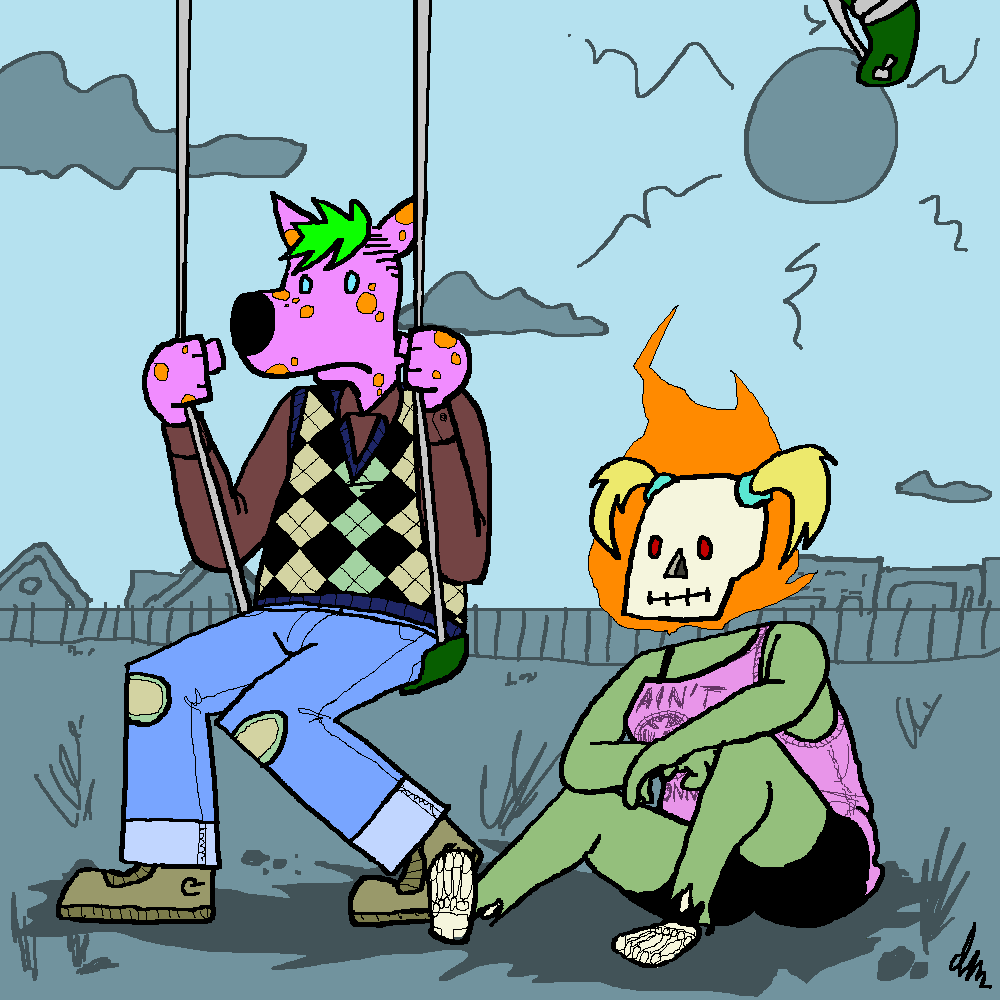
\includegraphics[width=.9\linewidth]{images/ref_IAN01}
  	\caption{Comic - \textit{Monster Friends in "Halloween"}}
  \label{fig:i1}
  \end{subfigure}
  \begin{subfigure}{.35\textwidth}
    \centering
    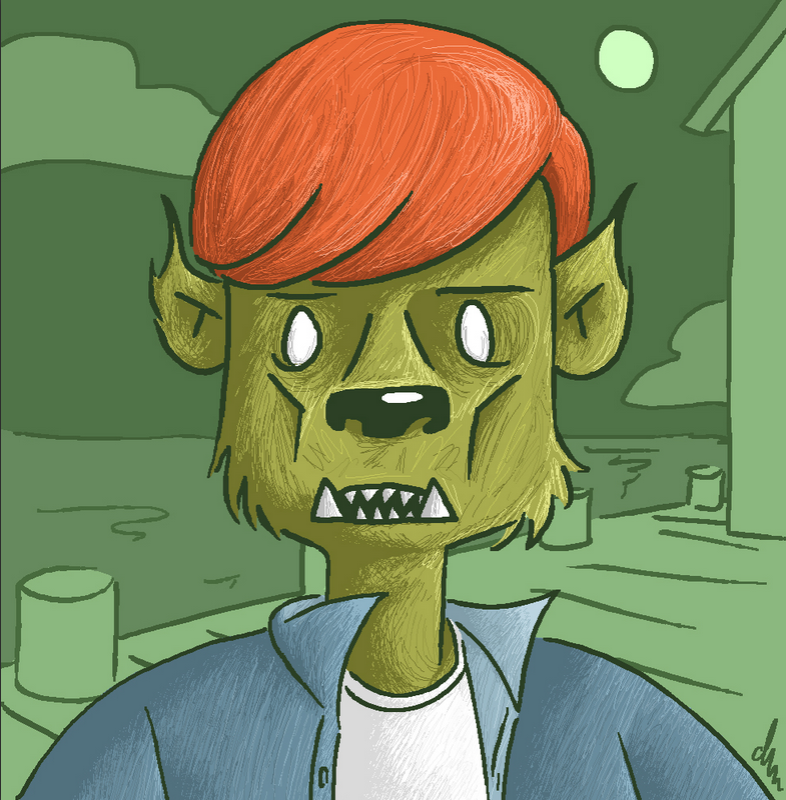
\includegraphics[width=.9\linewidth]{images/ref_IAN02}
  \end{subfigure}
  \begin{subfigure}{.3\textwidth}
    \centering
    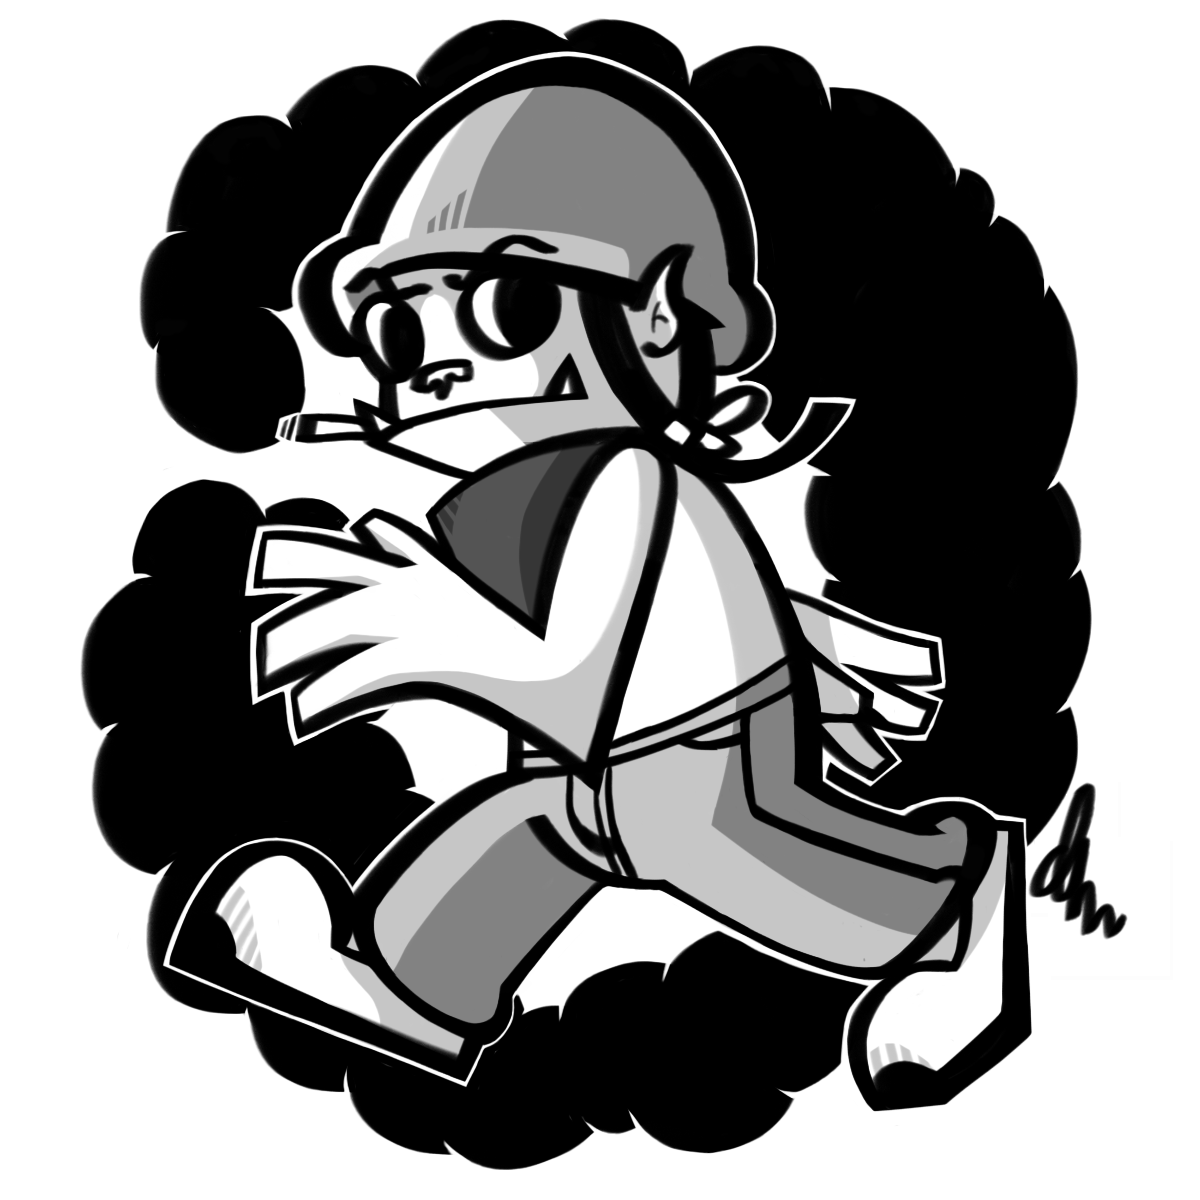
\includegraphics[width=.9\linewidth]{images/ref_IAN03}
  \end{subfigure}
  \begin{subfigure}{.4\textwidth}
    \centering
    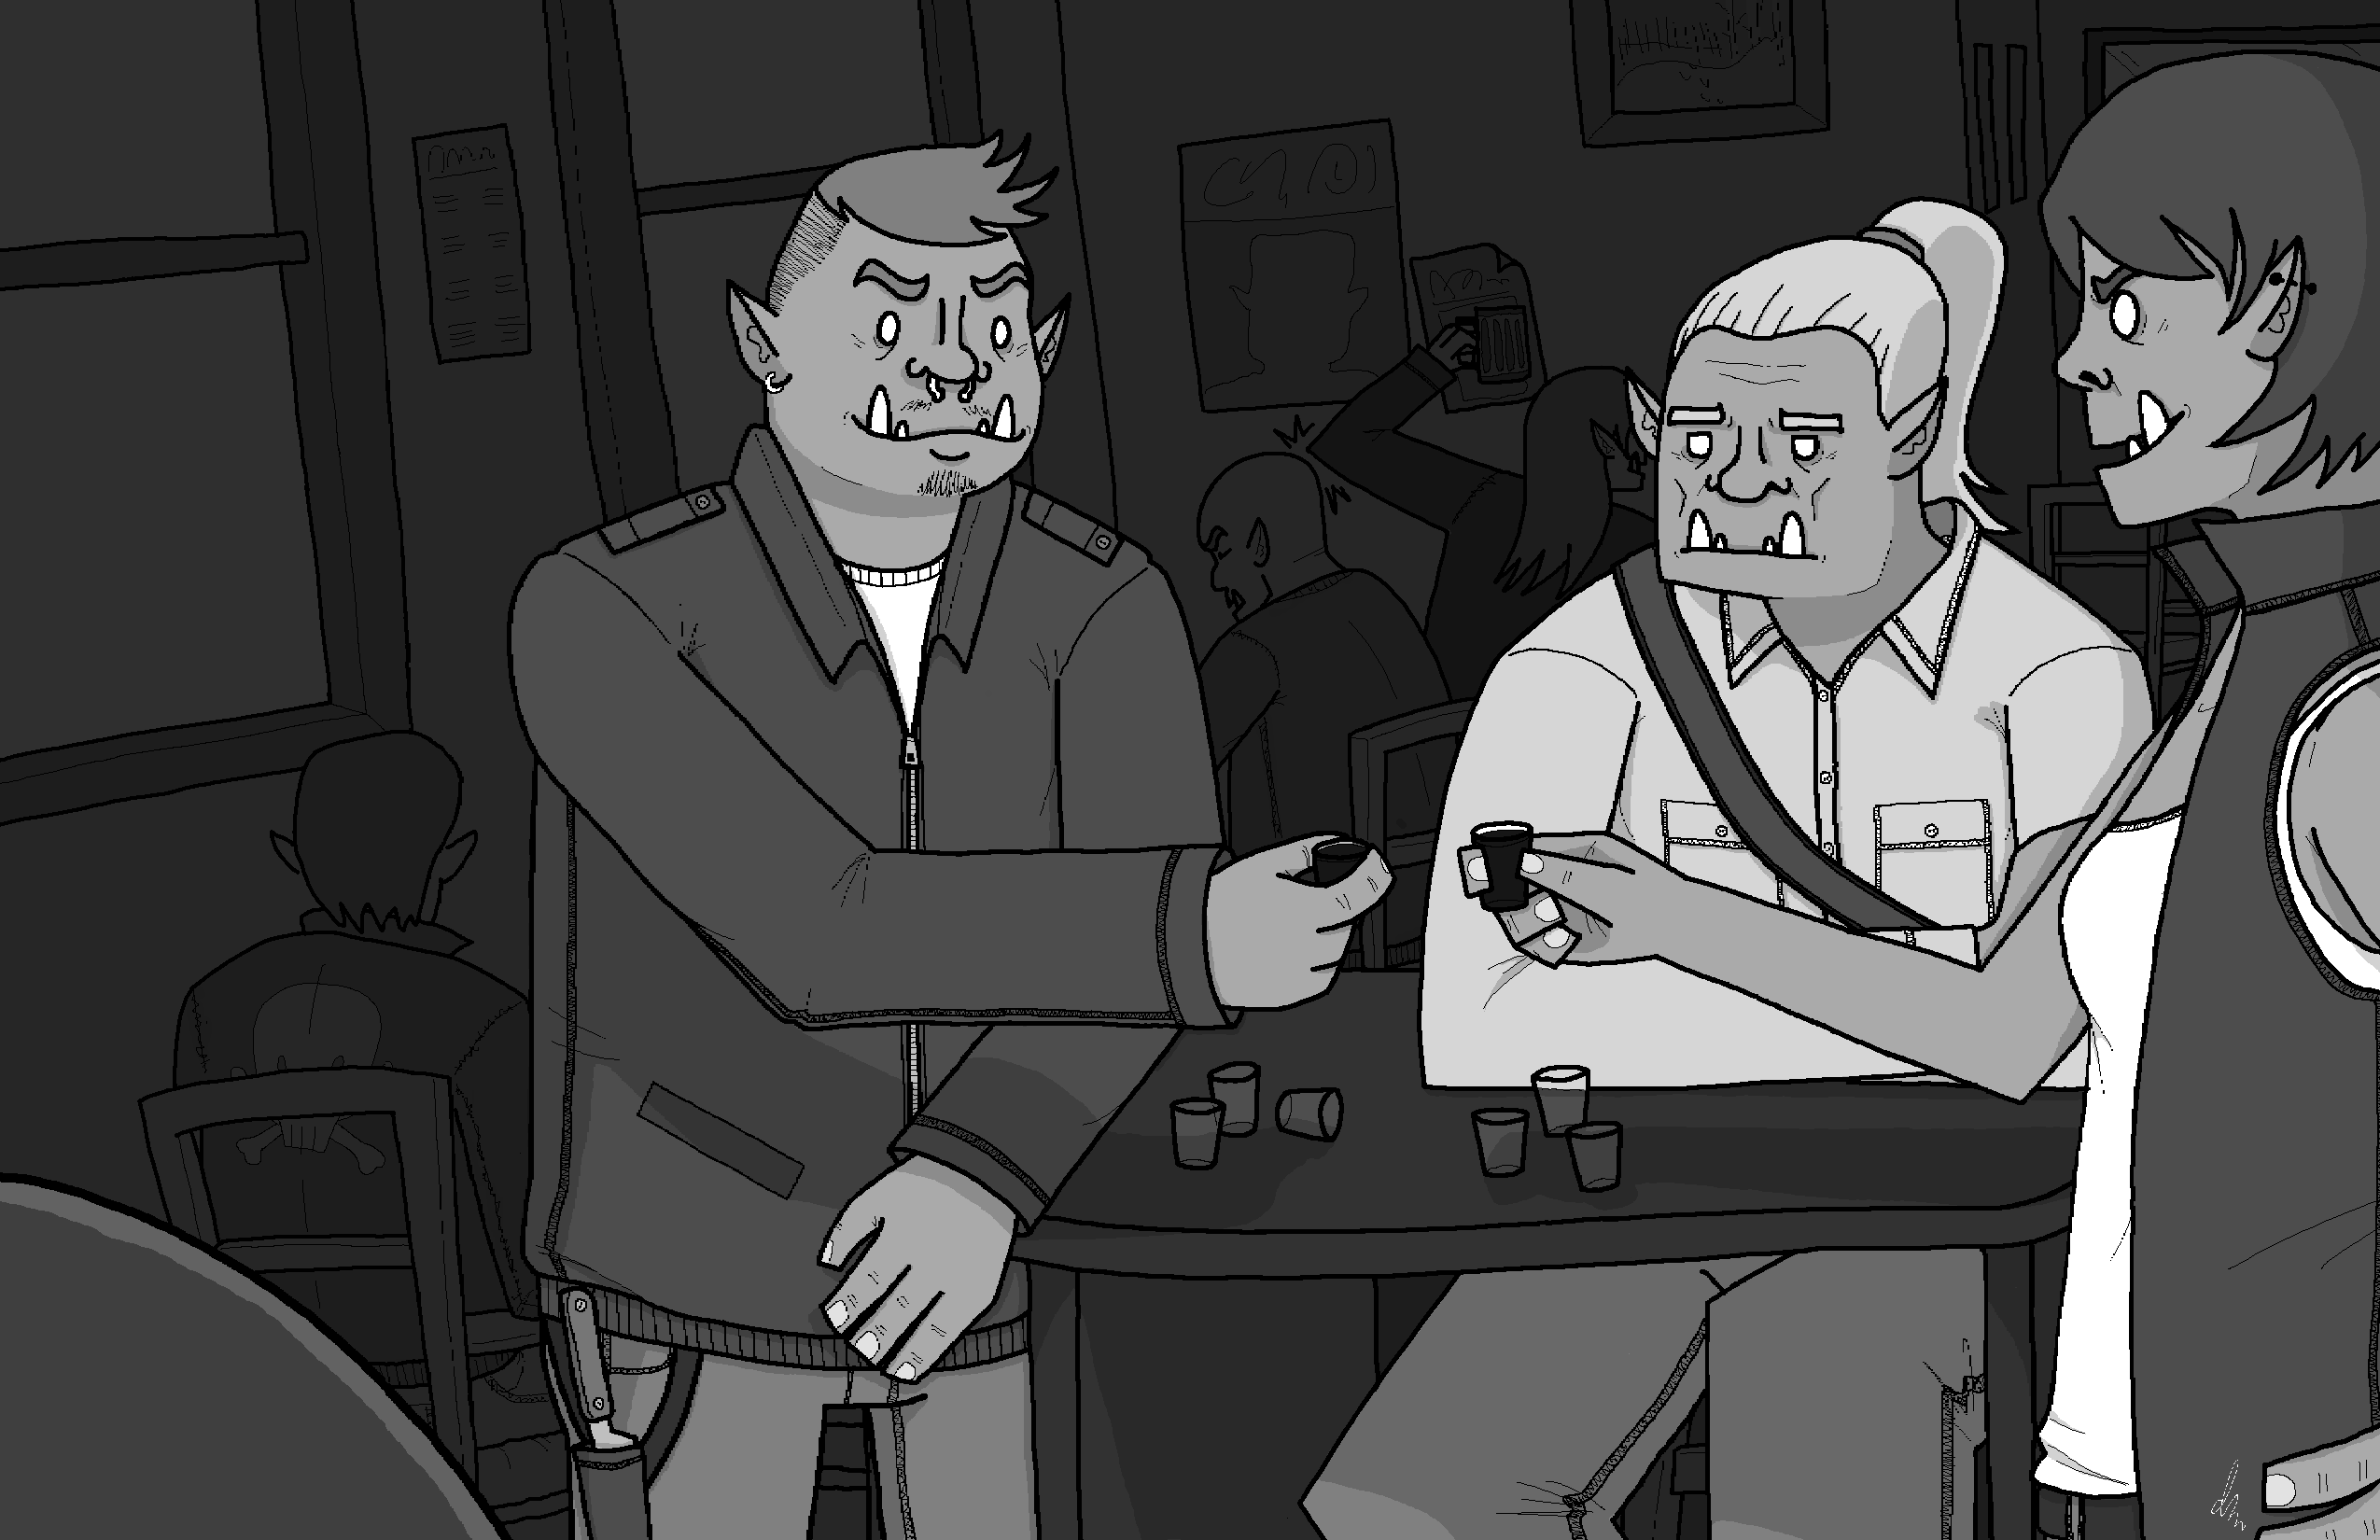
\includegraphics[width=.9\linewidth]{images/ref_IAN04}
  \end{subfigure}
  \caption{Ian's Art Style}
  \label{fig:istyle}
\end{figure}

\clearpage
\subsection{Catherine}
Catherine's artistic traits gravitate toward detailing and using subcultures as a point of reference. Her character designs ideas are typically human-based, their interests shown in their apparel and outward appearance. Certain shapes and colours are often used to accentuate the personality of the characters. She tends to focus on working with different clothing details and fashion aesthetics.

\begin{figure}[H]
  \centering\begin{subfigure}{.4\textwidth}
    \centering
    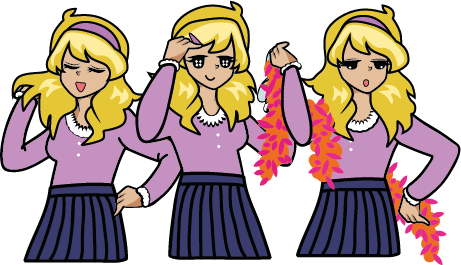
\includegraphics[width=.9\linewidth]{images/ref_CAT03}
  \end{subfigure}
  \begin{subfigure}{.4\textwidth}
    \centering
    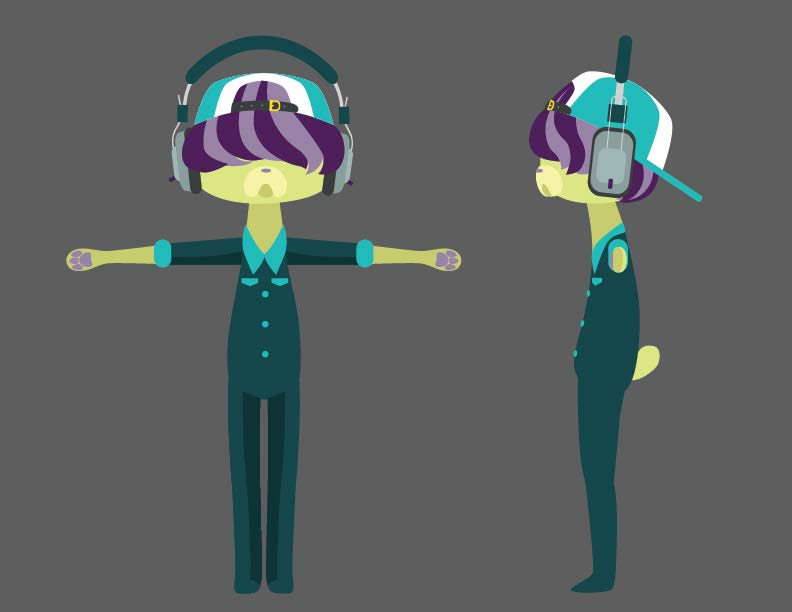
\includegraphics[width=.9\linewidth]{images/ref_CAT04}
  \end{subfigure}
  \begin{subfigure}{.3\textwidth}
    \centering
    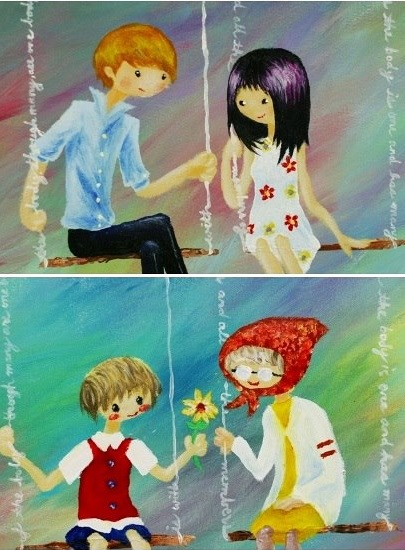
\includegraphics[width=.9\linewidth]{images/ref_CAT02}
  \end{subfigure}
  \begin{subfigure}{.6\textwidth}
    \centering
    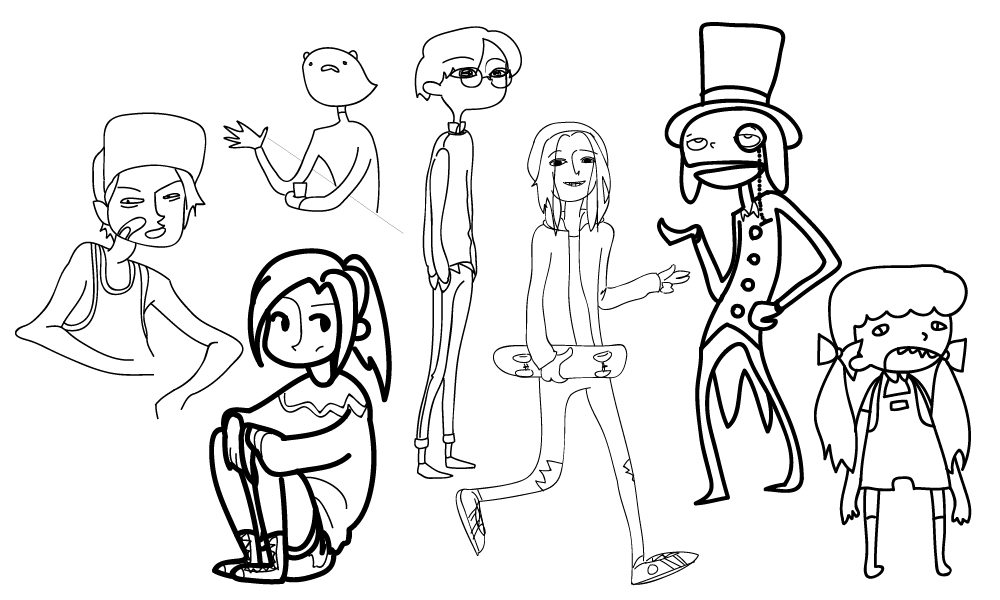
\includegraphics[width=.9\linewidth]{images/ref_CAT01}
  \end{subfigure}
  \caption{Cat's Art Style}
  \label{fig:cstyle}
\end{figure}